\section{The $\Z_2$-Homology Cover}
\label{sec:homcover}

Now, let~$G$ be directed, and let $h$
be a homology signature.  In this section, we describe an
algorithm to compute a $\Z_2$-minimal \emph{cycle} with signature~$h$
in $(g+b)^{O(g+b)}n \log n$ time. Our algorithm can be
used as a subroutine to compute minimum-cost even subgraphs in
\emph{any} homology class if the graph is undirected in the same asymptotic running time
using a dynamic programming procedure described later in this section.
Again, by Lemma~\ref{lem:surface-st-cut}, our algorithm can be used to find a minimum $s,t$-cut in~$G^*$ in the same amount of time if~$G$ is undirected.

The algorithm of the previous section constructs and searches several relevant finite portions of the (infinite) universal cover of the input surface.
Instead of the universal cover, the algorithms of this section construct and search another canonical covering space, called the \emph{$\Z_2$-homology cover}.
We also use a generalization of Klein's seminal multiple-source shortest path algorithm~\cite{k-msspp-05} for planar graphs to higher-genus embedded graphs \cite{cce-msspe-13}.
\note{TODO(kylejfox): The top of page 2 in the SODA 2011 paper contains some good motivation for the homology cover technique. That material should be transferred either to here or the introduction. Also mention the shortest non-trivial directed cycle papers~\cite{e-sncds-11,f-sntcd-13} that use similar techniques.}

\subsection{Constructing the $\Z_2$-homology cover}
\label{sec:homcover_cover}
After computing homology signatures for each edge, the $\Z_2$-homology cover of a combinatorial surface can be defined using a standard~\emph{voltage construction}~\cite[Chapter 4]{gt-tgt-01}, as follows.  Let $\Gbar$ denote the graph whose vertices are all ordered pairs $(v, h)$ where $v$ is a vertex of $G$ and $h$ is an element of $(\Z_2)^\beta$, and whose edges are the ordered pairs $(\arc{u}{v}, h) := (u, h)\arcto(v, h\oplus [u\arcto v])$ for all edges $\arc{u}{v}$ of $G$ and all homology classes $h \in (\Z_2)^\beta$.  Let $\pi\colon \Gbar\to G$ denote the covering map $\pi(v, h) = v$; this map projects any cycle in $\Gbar$ to a cycle in $G$.  To define a cellular embedding of~$\Gbar$, we declare a cycle in $\Gbar$ to be a face if and only if its projection is a face of $G$.  The combinatorial surface defined by this embedding is the $\Z_2$-homology cover $\Sigmabar$.

Our construction can be interpreted more topologically as follows.  Let $\dualarc_1, \dots, \dualarc_\beta$ denote the system of dual arcs used to define the homology signatures $[e]$.  The surface $D := \Sigma\setminus(\dualarc_1\cup\cdots\cup \dualarc_\beta)$ is a topological disk.  Each arc $\dualarc_i$ appears on the boundary of $D$ as two segments $\dualarc^+_i$ and~$\dualarc^-_i$.  For each signature $h\in (\Z_2)^\beta$, we create a disjoint copy $(D,h)$ of $D$; for each index~$i$, let $(\dualarc^+_i, h)$ and $(\dualarc^-_i, h)$ denote the copies of $\dualarc^+_i$ and $\dualarc^-_i$ in the disk $(D, h)$.  For each index~$i$, let~$b_i$ denote the $\beta$-bit vector whose $i$th bit is equal $1$ and whose other $\beta-1$ bits are all equal to~$0$.  The $\Z_2$-homology cover $\Sigmabar$ is constructed by gluing the~$2^\beta$ copies of $D$ together by identifying boundary paths $(\dualarc^+_i,h)$ and $(\dualarc^-_i, h\oplus b_i)$, for every index $i$ and homology class $h$.  See Figure \ref{fig:cover-ex} for an example.

\begin{figure}
\centering
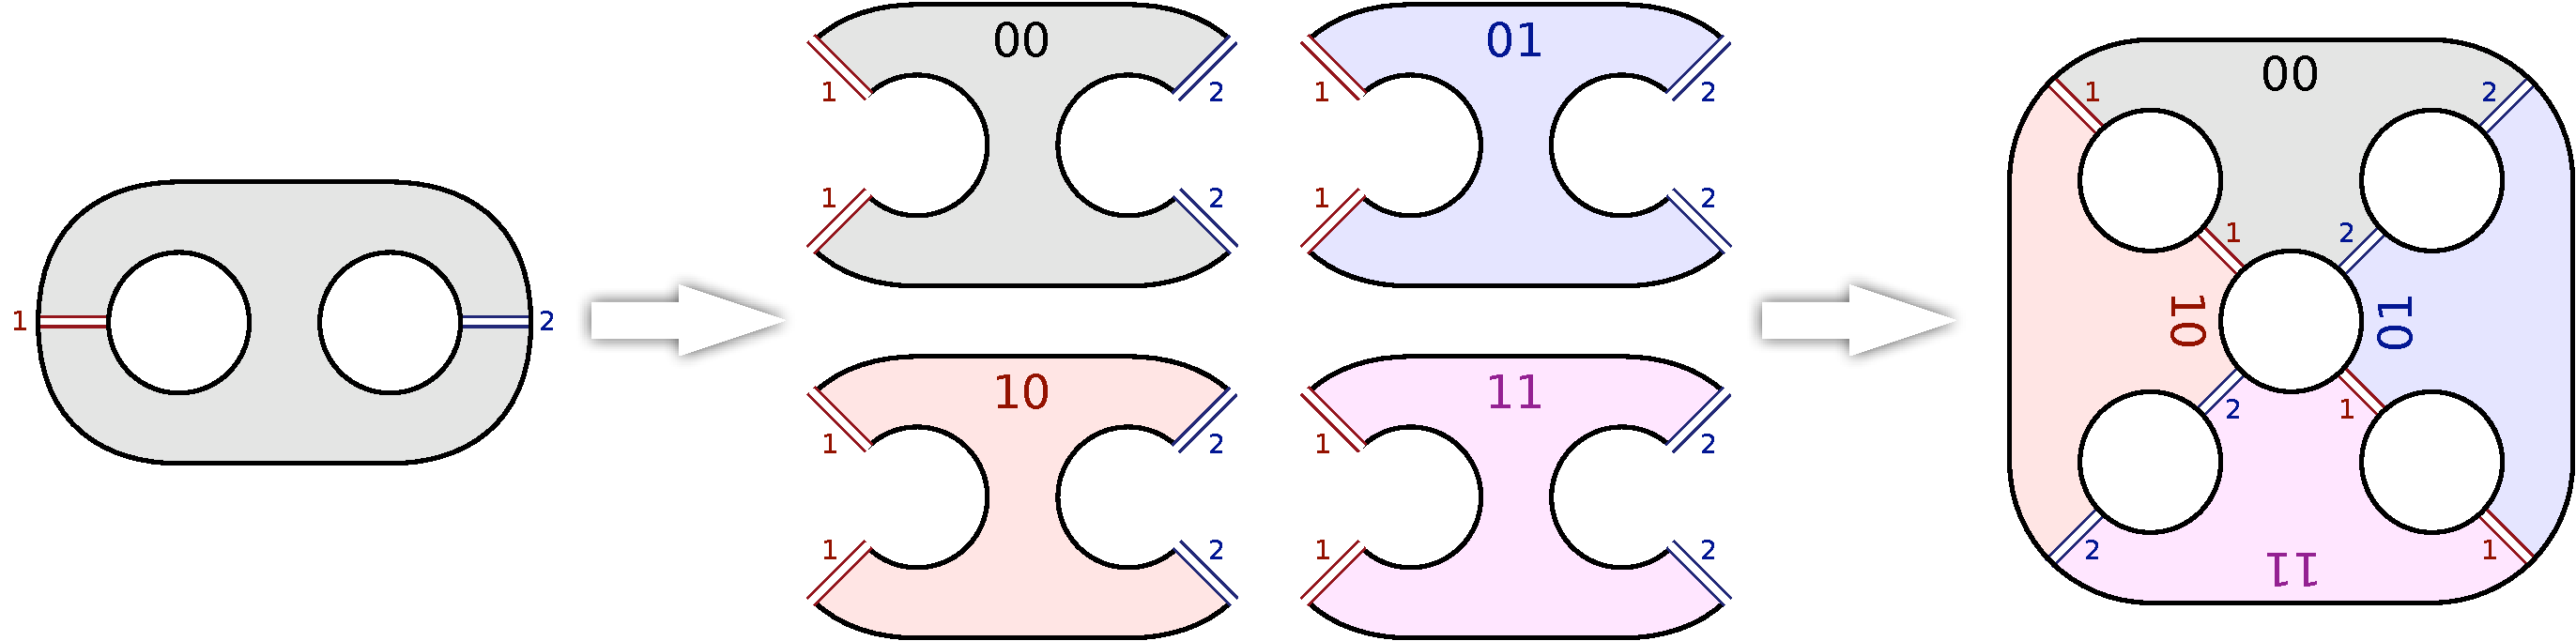
\includegraphics[height=1.5in]{Fig/hom-cover-example}
\caption{Constructing the $\Z_2$-homology cover of a pair of pants (a genus zero surface with three boundaries).}
\label{fig:cover-ex}
\end{figure}

\begin{lemma}
\label{lem:cover-cxy}
The combinatorial surface $\Sigmabar$ has $\nbar = 2^\beta n$ vertices, genus $\gbar = O(2^\beta \beta)$, and $\bbar = O(2^\beta b)$ boundaries, and it can be constructed in $O(2^\beta n)$ time.
\end{lemma}

\begin{proof}
Let $m$ and $f$ denote the number of edges and faces of $\Sigma$, respectively.  Recall that the Euler characteristic of $\Sigma$ is $\chi = n - m + f = 2 - 2g - b = 1-\beta$.  The combinatorial surface~$\Sigmabar$ has exactly $\nbar = 2^\beta n$ vertices, $2^\beta m$ edges, and $2^\beta f$ faces, so its Euler characteristic is $\chibar = 2^\beta (1-\beta)$.

If $b>1$, then each boundary cycle $\delta_i$ has a non-zero homology signature; at least one arc $\dualarc_j$ has exactly one endpoint on~$\delta_i$.  Thus, $\Sigmabar$ has exactly $\bbar = 2^{\beta-1} b$ boundary cycles, each of which is a double-cover (in fact, the $\Z_2$-homology cover) of some boundary cycle~$\delta_i$.  It follows that~$\Sigmabar$ has genus $\gbar = 1-(\chibar+\bbar)/2 = {2^{\beta-2} ({4g+b-4}) + 1}$.  (Somewhat surprisingly, $\Sigmabar$ may have positive genus even when $\Sigma$ does not!)  On the other hand, when $b=1$, the boundary cycle~$\delta_1$ is null-homologous, so $\Sigmabar$ has $\bbar = 2^\beta b$ boundary cycles, and thus~$\Sigmabar$ has genus $\gbar = {1-(\chibar+\bbar)/2} =  {2^\beta (g-1) + 1}$.

After computing the homology signatures for $\Sigma$ in $O(\beta n)$ time, following Lemma \ref{lem:sign}, it is straightforward to construct $\Sigmabar$ in $O(\nbar) = O(2^\beta n)$ time.
\end{proof}

We assign weights to the directed edges of $\Gbar$ by setting $\wbar(\arc{u}{v},h) := w(\arc{u}{v})$ for each edge $\arc{u}{v}$ of~$G$ and each homology class $h$.  In other words, each directed edge in $\Sigmabar$ inherits the weight of its projection in $\Sigma$.

Now consider an arbitrary path $\path$ in $G$, with (possibly equal) endpoints $u$~and $v$.  A straightforward induction argument implies that for any homology class $h \in (\Z_2)^\beta$, the path~$\path$ is the projection of a unique path from $(u,h)$ to $(v,h\oplus[\path])$, which we denote \EMPH{$(\path,h)$}.  Moreover, this lifted path has the same length as its projection: $w(\path) = \wbar(\path,h)$.  The following lemmas are now immediate.

\begin{lemma}
\label{lem:lift-shortest}
Every lift of a shortest directed path in $G$ is a shortest directed path in $\Gbar$.
\end{lemma}

\begin{lemma}
\label{lem:lift-minimal}
A loop $\ell$ in $G$ with basepoint $v$ is $\Z_2$-minimal if and only if, for every homology class $h\in (\Z_2)^\beta$, the lifted path $(\ell,h)$ is a shortest directed path in $\Gbar$ from $(v,h)$ to $(v,h\oplus[\ell])$.
\end{lemma}

% --------------------------------------------------------------------------------
\subsection{Computing $\Z_2$-minimal cycles}
\label{sec:homcover_cycles}

The results in the previous section immediately suggest an algorithm to compute the shortest directed cycle in a given $\Z_2$-homology class $h$ in time $2^{O(\beta)}n^2$: construct the $\Z_2$-homology cover, and then compute the shortest path from $(v,0)$ to $(v,h)$, for every vertex $v$ in the original graph.  In this section, we describe a more complex algorithm that runs in time $2^{O(\beta)}n\log n$.
Recall that any path $\sigma$ from $u$ to $v$ in $G$ is the projection of a unique path $(\sigma,0)$ from $(u,0)$ to $(v,[\sigma])$ in $\Gbar$.

\begin{lemma}
\label{lem:nocross}
Let $\cycle$ be a $\Z_2$-minimal cycle in $G$, and let~$\sigma$ be any shortest path in $G$ that intersects $\cycle$.  There is a $\Z_2$-minimal cycle $\cycle'$ homologous to $\cycle$, which is the projection of a shortest path $(\cycle', h)$ in $\Gbar$ that starts with a subpath of $(\sigma, 0)$ but does not otherwise intersect $(\sigma, 0)$.
\end{lemma}

\begin{proof}
Let $v$ be the vertex of $\sigma\cap\cycle$ closest to the starting vertex of $\sigma$, and let $(v,h)$ be the corresponding vertex of the lifted path $(\sigma,0)$.  Think of~$\cycle$ as a loop based at $v$.  Lemma \ref{lem:lift-minimal} implies that the lifted path $(\cycle, h)$ is a shortest path from $(v,h)$ to $(v,h\oplus [\cycle])$.

Now let $(w,h')$ be the last vertex along $(\cycle,h)$ that is also a vertex of $(\sigma,0)$.  Let $(\cycle', h)$ be the path obtained from $(\cycle, h)$ by replacing the subpath from from $(v,h)$ to $(w,h')$ with the corresponding subpath of $(\sigma,0)$.  By construction, $(\cycle', h)$ starts with a directed subpath of $(\sigma,0)$ but does not otherwise intersect $(\sigma,0)$.   Because both $(\cycle, h)$ and $(\sigma,0)$ are shortest paths in $\Sigmabar$, the new path $(\cycle', h)$ has the same length as $(\cycle, h)$.  Thus, the projected cycle $\cycle'$ has the same length and homology class as $\cycle$, which implies that~$\cycle'$ is $\Z_2$-minimal.
\end{proof}

We emphasize that the modified cycle $\cycle'$ may intersect~$\sigma$ arbitrarily many times; however, all such intersections lift to intersections between $(\cycle', h)$ and lifts of $\sigma$ other than $(\sigma, 0)$.

Our algorithm uses a generalization of Klein's seminal multiple-source shortest path algorithm~\cite{k-msspp-05} to higher-genus embedded graphs:

\begin{lemma}[Chambers \etal~\cite{cce-msspe-13}]
\label{lem:multishort}
Let $G$ be a directed graph with non-negative edge weights, cellularly embedded on a surface $\Sigma$ of genus $g$ with $b>0$ boundaries, and let $f$ be an arbitrary face of $G$.  We can preprocess $G$ in $O(gn\log n)$ time and $O(n)$ space so that the length of the shortest path from any vertex incident to $f$ to any other vertex can be retrieved in $O(\log n)$ time.
\end{lemma}

\begin{theorem}
\label{thm:min-cycle}
Let $G$ be a directed graph with non-negative edge weights, cellularly embedded on a surface~$\Sigma$ with first Betti number $\beta$, and let~$\cycle$ be a cycle in~$G$ with $k$ edges.  A shortest directed cycle in~$\Sigma$ that is $\Z_2$-homologous with~$\cycle$ can be computed in $O(\beta k + 4^\beta \beta^2\, n\log n)$ time.
\end{theorem}

\begin{proof}
We begin by computing homology signatures for the edges of $G$ in $O(\beta n)$ time, as described in Section~\ref{sec:characterizing_signatures}.  In $O(\beta k)$ time, we then compute the homology signature~$[\cycle]$.  If $[\cycle] = 0$, we return the empty walk and halt.

Next, we construct the $\Z_2$-homology cover $\Gbar$ in $O(2^\beta n\log n)$ time, as described in Section~\ref{sec:homcover_cover}, as well as the set $S$ of directed shortest paths described in Section~\ref{sec:characterizing_crossings}.
Any cycle homologous with~$\cycle$ must intersect at least one member of~$S$ as if~$\cycle$ is not null-homologous.
We look for the shortest path in $\Gbar$ of the canonical form described in Lemma~\ref{lem:nocross}, by considering each shortest path $\sigma\in S$ in turn as follows.

Let us write $(\sigma,0) = (v_0,0) \arcto (v_1,h_1) \arcto\allowbreak \cdots\arcto (v_t, h_t)$.  We construct the combinatorial surface $\Sigmabar\snip(\sigma,0)$ by splitting the path $(\sigma,0)$ into two parallel paths from $(v_0,0)$ to $(v_t,h_t)$, which we denote  $(\sigma,0)^+$ and $(\sigma,0)^-$.  For each index $1\le i\le t-1$, let $(v_i,h_i)^+$ and $(v_i,h_i)^-$ denote the copies of vertex $(v_i,h_i)$  on the paths $(\sigma,0)^+$ and $(\sigma,0)^-$, respectively.  The paths $(\sigma,0)^+$ and $(\sigma,0)^-$ bound a new common face $f_{(\sigma,0)}$ in $\Sigmabar\snip(\sigma,0)$.

Lemma \ref{lem:nocross} implies that if any $\Z_2$-minimal cycle homologous to $\cycle$ intersects $\sigma$, then some $\Z_2$-minimal cycle homologous to $\cycle$ is the projection of a shortest path in $\Sigmabar\snip(\sigma,0)$ from some vertex $(v_i,h_i)^\pm$ to the corresponding vertex $(v_i, h_i\oplus[\cycle])$.  To compute these shortest paths, we implicitly compute the shortest path in $\Sigmabar\snip(\sigma,0)$ from every vertex on the boundary of $f_{(\sigma,0)}$ to \emph{every} vertex of $\Sigmabar\snip(\sigma,0)$, using Lemma~\ref{lem:multishort}.  The resulting algorithm runs in $O(\gbar\,\nbar \log \nbar) = O(4^\beta \beta^2\, n\log n)$ time, by Lemma \ref{lem:cover-cxy}.
\end{proof}

By running this algorithm $2^\beta$ times, we can compute the shortest directed cycle in $\Sigma$ in \emph{every} $\Z_2$-homology class, in $O(8^\beta \beta^2\, n\log n)$ time.  In particular, we can compute the shortest directed cycle in~$\Sigma$ that has nontrivial $\Z_2$-homology.  When the original surface has no boundary, this is just the shortest \emph{non-separating} cycle in $\Sigma$.  Recently, Cabello \etal~\cite{ccl-fsncd-10} described an algorithm to compute the shortest non-separating cycle in any surface-embedded directed graph in $O(g^{1/2} n^{3/2}\log n)$ time; our algorithm is faster whenever $g \le (\lg n)/13$.

\begin{corollary}
\label{C:nonsep}
Given a directed graph $G$ with $n$ vertices with non-negative edge weights, cellularly embedded on a surface with genus~$g$, we can compute the shortest directed cycle in $G$ that is non-separating in $\Sigma$ in $O(64^g g^2 n\log n)$ time.
\end{corollary}

Note however, that a recent algorithm of Erickson~\cite{e-sncds-11} improves this running time further to~$O(g^2 n \log n)$ by using similar similar techniques in a different covering space known as the cyclic double cover.
Cabello \etal~\cite{ccl-fsncd-10} also described an algorithm to find the shortest \emph{non-contractible} cycle in an embedded directed graph in $O(g^{1/2} n^{3/2}\log n)$ time.  Our approach does not lead to a faster algorithm for this problem;  contractibility is inherently  a property of \emph{homotopy}, not homology.

% --------------------------------------------------------------------------------
\subsection{Minimum cuts from the homology cover}
\label{sec:homcover_mincut}

We now apply our algorithm for computing $\Z_2$-minimal cycles to the problem of computing $\Z_2$-minimal even subgraphs in \emph{undirected} surface embedded graphs.
\note{TODO(kylejfox): Emphasize here or in the intro that we cannot use these techniques to do directed minimum cut.}
Theorem~\ref{thm:min-cycle} immediately implies that we can compute a minimum-weight \emph{cycle} in every $\Z_2$-homology class in $O(8^\beta \beta^2\, n\log n)$ time.  However, the minimum weight \emph{even subgraph} in a given homology class may not be (the carrier of) a $\Z_2$-minimal cycle.  In particular, if a $\Z_2$-minimal cycle $\gamma$ traverses any edge more than once, then every minimum-weight even subgraph with signature $[\gamma]$ \emph{must} be disconnected.

However, any \emph{connected} $\Z_2$-minimal even subgraph is the carrier of a $\Z_2$-minimal cycle, and the components of any $\Z_2$-minimal even subgraph are themselves $\Z_2$-minimal even subgraphs.  Thus, we can assemble a $\Z_2$-minimal even subgraph in any homology class from a subset of the $\Z_2$-minimal cycles we have already computed.  The following lemma puts an upper bound on the number of cycles we need.

\begin{lemma}
\label{lem:even-comps}
Every $\Z_2$-minimal even subgraph of $G$ has at most $g+b-1$ components.
\end{lemma}

\begin{proof}
Let $\gamma_1, \dots, \gamma_{g+b}$ be disjoint simple cycles on an \emph{abstract} surface $\Sigma$ of genus $g$ with $b$ boundaries, and consider the surface $\Sigma' = \Sigma \setminus (\gamma_1 \cup \cdots \cup \gamma_{g+b})$.  The definition of genus implies that $\Sigma'$ cannot be connected; indeed, $\Sigma'$ must have at least $b+1$ components.  So the pigeonhole principle implies that some component $\Sigma''$ of~$\Sigma$ does not contain any of the boundary cycles of $\Sigma$.  The boundary of $\Sigma''$ is therefore null-homologous.

Now let $\eta$ be an even subgraph of $G$ with more than $g+b-1$ components.  Each component has a cycle decomposition, so $\eta$ must have a cycle decomposition with more than $g+b-1$ elements.  Thus, the argument in the first paragraph implies that some subgraph of $\eta$ must be null-homologous.  We conclude that $\eta$ is not $\Z_2$-minimal.
\end{proof}

\begin{theorem}
\label{thm:min-even}
Let $G$ be an \textbf{undirected} graph with non-negative edge weights, cellularly embedded on a surface~$\Sigma$ with first Betti number $\beta$.  A minimum-weight even subgraph of $G$ in each $\Z_2$-homology class can be computed in $O(8^\beta \beta^2\, n\log n)$ time.
\end{theorem}

\begin{proof}
Our algorithm computes a minimum-weight cycle~$\gamma_h$ in every $\Z_2$-homology class~$h$ in $O(8^\beta \beta^2\, n\log n)$ time, via Theorem \ref{thm:min-cycle}, and then assembles these $\Z_2$-minimal cycles into $\Z_2$-minimal even subgraphs using dynamic programming.

For each homology class $h\in (\Z_2)^\beta$ and each integer $1\le k\le g+b-1$, let \EMPH{$C(h,k)$} denote the minimum total weight of any set of at most $k$ cycles in $G$ whose homology classes sum to $h$.  Lemma~\ref{lem:even-comps} implies that the minimum weight of any even subgraph in homology class~$h$ is exactly $C(h, g+b-1)$.  This function obeys the following straightforward recurrence:
\[
	C(h,k) = \min\Setbar{C(h_1,k-1) + C(h_2, 1)}{h_1\oplus h_2 = h}.
\]
This recurrence has two base cases: $C(0, k) = 0$ for any integer $k$, and for any homology class $h$, the value $C(h,1)$ is just the length of $\gamma_h$.  A standard dynamic programming algorithm computes $C(h, g+b-1)$ for all $2^\beta$ homology classes $h$ in $O(4^\beta \beta)$ time.  We can then assemble the actual minimum-weight even subgraphs in each homology class in $O(\beta n)$ time.  The total time for this phase of the algorithm is $O(4^\beta \beta + 2^\beta \beta n)$, which is dominated by the time to compute all the $\Z_2$-minimal cycles.
\end{proof}

\begin{corollary}
\label{cor:mincut}
Let $G$ be an edge-weighted undirected graph embedded on a surface with genus $g$ and $b$ boundary components, and let $s$ and $t$ be vertices of $G$.  We can compute the minimum-weight $(s,t)$-cut in $G$ in $O(16^g g^2 n \log n)$ time.
\end{corollary}
